%  article.tex (Version 3.3, released 19 January 2008)
%  Article to demonstrate format for SPIE Proceedings
%  Special instructions are included in this file after the
%  symbol %>>>>
%  Numerous commands are commented out, but included to show how
%  to effect various options, e.g., to print page numbers, etc.
%  This LaTeX source file is composed for LaTeX2e.

%  The following commands have been added in the SPIE class 
%  file (spie.cls) and will not be understood in other classes:
%  \supit{}, \authorinfo{}, \skiplinehalf, \keywords{}
%  The bibliography style file is called spiebib.bst, 
%  which replaces the standard style unstr.bst.  

\documentclass[]{spie}  %>>> use for US letter paper
%%\documentclass[a4paper]{spie}  %>>> use this instead for A4 paper
%%\documentclass[nocompress]{spie}  %>>> to avoid compression of citations
%% \addtolength{\voffset}{9mm}   %>>> moves text field down
%% \renewcommand{\baselinestretch}{1.65}   %>>> 1.65 for double spacing, 1.25 for 1.5 spacing 
%  The following command loads a graphics package to include images 
%  in the document. It may be necessary to specify a DVI driver option,
%  e.g., [dvips], but that may be inappropriate for some LaTeX 
%  installations. 
\usepackage[]{graphicx}
\usepackage{caption} 
\usepackage{subcaption} 
\usepackage{hyperref}
%\usepackage{mathtools}

\title{CT Thermometry for Cone-beam CT Guided Ablation} 

%>>>> The author is responsible for formatting the 
%  author list and their institutions.  Use  \skiplinehalf 
%  to separate author list from addresses and between each address.
%  The correspondence between each author and his/her address
%  can be indicated with a superscript in italics, 
%  which is easily obtained with \supit{}.

\author{Zachary DeStefano\supit{a}, Nadine Abi-Jaoudeh\supit{b}, Ming Li\supit{c}, Bradford J Wood\supit{b}, Ronald M Summers\supit{a}, Jianhua Yao\supit{a}
\skiplinehalf
\supit{a}Clinical Image Processing Services, Radiology and Imaging Sciences, \\Clinical Center, National Institutes of Health, Bethesda, MD 20892\\
\supit{b}Interventional Radiology, Radiology and Imaging Sciences, \\Clinical Center, National Institutes of Health, Bethesda, MD 20892\\
\supit{c}National Heart, Lung and Blood Institute, \\National Institutes of Health, Bethesda, MD, USA
}

%>>>> Further information about the authors, other than their 
%  institution and addresses, should be included as a footnote, 
%  which is facilitated by the \authorinfo{} command.

%\authorinfo{Author Emails: zdestefa@uci.edu, abijaoudehn@cc.nih.gov, ,bwood@nih.gov}
%%>>>> when using amstex, you need to use @@ instead of @
 

%%%%%%%%%%%%%%%%%%%%%%%%%%%%%%%%%%%%%%%%%%%%%%%%%%%%%%%%%%%%% 
%>>>> uncomment following for page numbers
% \pagestyle{plain}    
%>>>> uncomment following to start page numbering at 301 
%\setcounter{page}{301} 
 
  \begin{document} 
  \maketitle 

%%%%%%%%%%%%%%%%%%%%%%%%%%%%%%%%%%%%%%%%%%%%%%%%%%%%%%%%%%%%% 
\begin{abstract}

Monitoring temperature during a cone-beam CT (CBCT) guided ablation procedure is important for prevention of over-treatment and under-treatment. In order to accomplish ideal temperature monitoring, a thermometry map must be generated. Previously, this was attempted using CBCT scans of a pig shoulder undergoing ablation. We are extending this work by using CBCT scans of real patients and incorporating more processing steps. We register the scans before comparing them due to the movement and deformation of organs. We then automatically locate the needle tip and the ablation zone. We employ a robust change metric due to image noise and artifacts. This change metric takes windows around each pixel and uses an equation inspired by Time Delay Analysis to calculate the error between windows with the assumption that there is an ideal spatial offset. Once the change map is generated, we correlate change data with measured temperature data at the key points in the region. This allows us to transform our change map into a thermal map. This thermal map is then able to provide an estimate as to the size and temperature of the ablation zone. We evaluated our procedure on a data set of 12 patients who had a total of 24 ablation procedures performed. We were able to generate reasonable thermal maps with varying degrees of accuracy. The average error ranged from 2.7 to 16.2 degrees Celsius. In addition to providing estimates of the size of the ablation zone for surgical guidance, 3D visualizations of the ablation zone and needle are also produced.
\end{abstract}

%>>>> Include a list of keywords after the abstract 

\keywords{Cone-beam CT, CBCT, Thermometry, Radiofrequency Ablation, Time Delay Analysis}

\section{Introduction}
\label{sec:intro}  % \label{} allows reference to this section

Radiofrequency ablation (RFA) has become a common interventional procedure for treating cancerous tumors in various parts of the body \cite{Mayo15}. C-arm Cone-beam CT (CBCT) is an imaging modality that has been adopted for a variety of purposes\cite{Orth08}, including guidance during RFA. We still however have difficulty determining how much tissue has been affected by the procedure. Specifically, we need to know the temperature changes that have occurred in the tissue\cite{Li13}. We want to make sure only the cancerous tissue has been heated and not the healthy tissue. Ideally, each of the CBCT voxels would also have a temperature reading. We would then be able to superimpose the thermal volume on the CBCT scan and quickly find out which tissue has been affected.

This possibility has been explored in the past \cite{Li13} but only for phantoms. We decided to extend the work to real patients and incorporate more processing steps to enhance the thermal maps. For this work, we had a data set of CBCT scans taken during RFA procedures. With each procedure, there was a baseline CBCT scan taken after the ablation needle was inserted but before it was heated. There were then 1-4 comparison scans taken as the needle was heated and cooled. We processed each of the comparison scans and attempted to generate a thermal map by comparing them to the baseline scan.

\section{Method}

Before we starting analyzing the values, we registered the CBCT scans together using an open source software package known as NiftyReg \cite{Modat10}. We then processed the CBCT scan data in the ROI where the ablation occurred. There is strong evidence that the relationship between HU unit and temperature is linear \cite{Fani14} thus we correlated change in HU with change in temperature. We then used this model to generate the thermal map. The change value we used was not simple HU difference, but a technique entitled Spatial Offset RMSE that is more robust to noise and artifacts. 

With this technique, for each pixel, we calculated the minimum RMSE between the baseline and comparison windows assuming that there is a spatial offset between them. For each pixel, let $U$ be the $n$ by $n$ window around it in the baseline image and let $V$ be the $n$ by $n$ window around it in the comparison image. We made the matrix $U'$ which is $U$ repeated in the following manner:
\[
\forall(k,l,i \in Z)\, \, \, U'_{k+i \cdot n,l+i \cdot n} = U_{k,l}
\]
Afterward the following was calculated and the value was stored as the pixel value in the result image:
\[
\min_{r,c} \sqrt{ \frac{1}{n^2} \sum_{l=0}^{n-1} \sum_{k=0}^{n-1} {(U'_{k+r,l+c}-V_{k,l})^2}}
\]
Figure \ref{changeDetectionMethods} shows how our metric outperforms the raw difference method and the filtered difference (difference of slices after they are filtered via convolutional averaging) method. 

\begin{figure} 
\centering 
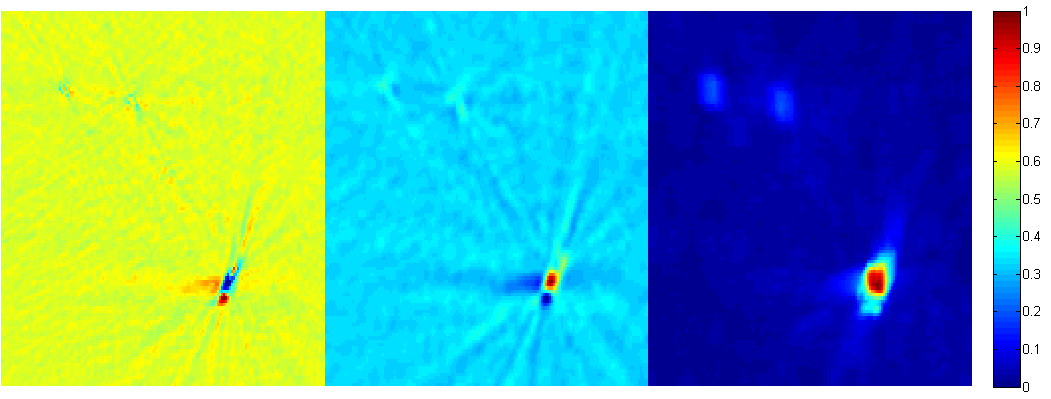
\includegraphics[width=\textwidth]{changeDetectionPanel2.png} 
\caption{Results of different change metrics in the ROI. Raw subtraction (left), Filtered Difference (center), and Spatial Offset RMSE (right). Each image is normalized in order to show how the thermal map would appear} 
\label{changeDetectionMethods}
\end{figure}

\section{Results}

We used a data set of CBCT scans taken for 13 patients whose procedures were performed between September 2013 and June 2015. For each patient, there were between 1 and 4 ablations done. With each ablation, a baseline scan was taken followed by 1-4 comparison scans at different time points. Each of these time points had the ablation needle at different temperatures. We generated a thermal map at each of these time points in order to estimate the amount of tissue affected. 

\subsection{Finding Error Rates}

We decided to take the thermal maps generated from regression and see the average temperature in the zones that we were testing. We then did an RMSE of those temperatures with the measured temperatures. We divided this RMSE by the temperature range in order to obtain an error ratio. The results are in table 1. In the table, temperatures are in Celsius and \textit{Temps (From Regression)} is the average temperature in the neighborhood around the needle or thermocouple (with radius specified by \textit{Neighborhood Radius}) in the thermal map calculated from regression. Our error rate ranged from 8-22\% and the error amount ranged range 2.7 to 16.2 degrees Celsius. 

\begin{tabular}{ | l | l | l | l | l | l | l | }
\hline
	Pt Num & 4 & 5 & 5 & 6 & 8 & 9 \\ \hline
	Procedure Num & 1 & 1 & 3 & 1 & 1 & 1 \\ \hline
	Pt Sex & M & M & M & F & F & F \\ \hline
	Pt Age & 54 & 48 & 48 & 65 & 59 & 61 \\ \hline
	 &  &  &  &  &  &  \\ \hline
	Baseline Temps & 36/36 & 35/35 & 38/36 & 31/31/30 & 36/37 & 37/37 \\ \hline
	 &  &  &  &  &  &  \\ \hline
	Comparison 1 &  &  &  &  &  &  \\ \hline
	Temps (Given) & 64/56 & 58/38 & 48/83 & 132/124/45 & 100/37 & 145/42 \\ \hline
	Temps (From Regression) & 67.2/59.6 & 64.2/45.4 & 50.9/62.2 & 128.4/108.9/81.0 & 111.0/36.6 & 142.6/56.5 \\ \hline
	 &  &  &  &  &  &  \\ \hline
	Comparison 2 &  &  &  &  &  &  \\ \hline
	Temps (Given) & 67/57 & 66/58 & 52/95 & 126/107/98 & 52/38 & 47/37 \\ \hline
	Temps (From Regression) & 65.5/59.2 & 66.0/46 & 66.8/94.7 & 126.7/110.0/103.1 & 65.2/36.5 & 50.7/55.6 \\ \hline
	&  &  &  &  &  &  \\ \hline
	Given \& Regression Temp RMSE & 2.752 & 7.7 & 12.847 & 16.189 & 8.626 & 11.997 \\ \hline
	Error Ratio & 8.8774E-2 & 0.2484 & 0.2177 & 0.1587 & 0.2396 & 0.1110 \\ \hline
\end{tabular}
 

\subsection{Approximating Ablation Zone Area}

After generating a thermal map, we identified the point with the highest temperature as being the likely center of ablation. We then made a graph showing the average temperature in a region around that point as a function of the radius of the region. We can potentially use the values of the function to approximate the radius of the ablation zone. Once the average is below a certain fixed temperature or below a certain percentage of the peak, we are outside the ablation zone. Figure \ref{graphRadMean} shows these values for various patients in our study. 

\begin{figure} 
\centering 
\begin{subfigure}[t]{.4\textwidth} 
	\centering 
	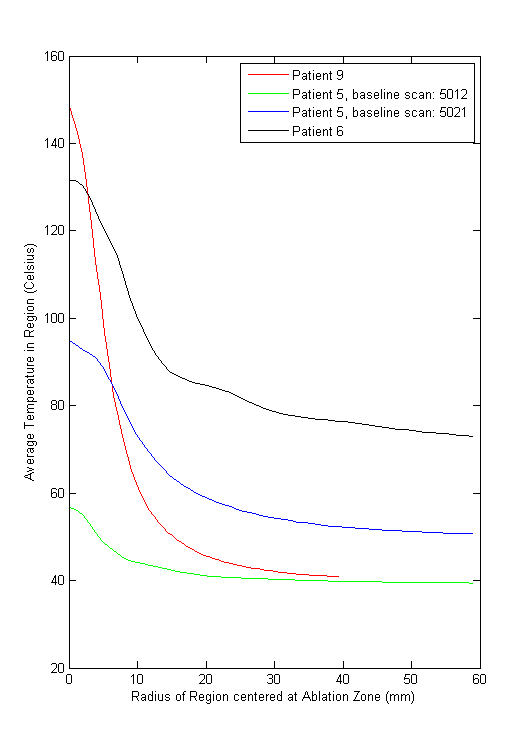
\includegraphics[width=\textwidth,height=4in]{meanTempVsRadiusFull.png} 
	\caption{Graph of radius vs mean temperature} 
	\label{graphRadMean}
\end{subfigure}
\begin{subfigure}[t]{.4\textwidth} 
	\centering 
	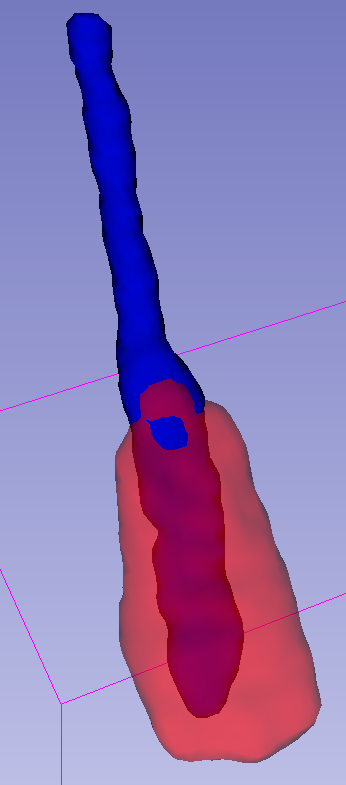
\includegraphics[width=\textwidth,height=4in]{NeedleAndAblationZone.png} 
	\caption{3D Visualization of the Needle and Ablation Zone}
	\label{needleAblationZone} 
\end{subfigure}

\end{figure}


\subsection{3D Visualization of Ablation Zone}

We were able to produce a 3D visualization of the needle and the ablation zone. We thresholded the values of the 3D Thermal Map generated which produced a binarized 3D volume. We also thresholded the values of the original CBCT scan in order to produce a binarized 3D volume showing only the needle. With both volumes, we ran a surface generation algorithm using \href{www.itksnap.org}{ITK-SNAP} \cite{Yushkevich06}. This created two 3D meshes. We superimposed them in \href{http://www.slicer.org/}{3D Slicer} \cite{Fedorov12} to show the needle and ablation zone together. Figure \ref{needleAblationZone} displays the result.

\section{Conclusions}

The processing steps we performed seem to be good initial steps toward incorporating CT Thermometry in clinical practice. Affine and Deformable Registration aligned the CBCT scans allowing us a much more accurate change map. Needle Detection provided a quick way of finding the ROI. The change metric we used provided smooth change maps that were able to generate reasonable thermal maps. 

For some of the patients, these thermal maps were quite accurate while for others the error was higher. The higher error was the result of a high residual value in the linear regression. This was likely caused by image noise or registration error. In the cases where the error was low, the thermal maps have the potential to be quite useful during ablation procedures. They may be used to approximate the size of the ablation zone. Additionally, there is the potential to generate a 3D visual representation of the ablation zone. 

\bibliography{report}   %>>>> bibliography data in report.bib
\bibliographystyle{spiebib}   %>>>> makes bibtex use spiebib.bst

\end{document} 
